%%%%%%%%%%%%%%%%%%%%%%%%%%%%%%%%%%%%%%%%%%%%%%%%%%%%%%%%%%%%%%%%%%%%%%%%%%%%%%%%
\chapter{Системотехническая часть}
%%%%%%%%%%%%%%%%%%%%%%%%%%%%%%%%%%%%%%%%%%%%%%%%%%%%%%%%%%%%%%%%%%%%%%%%%%%%%%%%

%%%%%%%%%%%%%%%%%%%%%%%%%%%%%%%%%%%%%%%%%%%%%%%%%%%%%%%%%%%%%%%%%%%%%%%%%%%%%%%%
\section{Анализ предметной области}
\subsection{Интерактивное обучение}
Сам термин «обучение» может трактоваться в педагогике достаточно широко. Одно из наиболее удачных определений звучит так:
обучение — это двусторонний процесс, осуществляемый учителем (преподавание) и учащимся (учение) \cite{pedDict}.

В данном контексте необходимо разграничить понятия «обучение» и «познание». Так, первичным относительно процесса обучения является отношение «обучающий — обучаемый», которое порождает отношение «обучаемый — учебный материал», относящееся в свою очередь уже к понятию «познание». То есть, ключевым процессом является процесс познания, а обучение — это часть процесса познания, для которой необходимо наличие учителя.

Схематично модель процесса обучения приведена на рисунке \ref{fig:ed-process}

\begin{figure}[htbp]
\centering
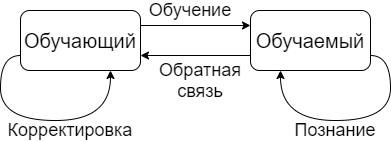
\includegraphics[width=\textwidth]{ed-process.png}
\caption{Модель процесса обучения}%
\label{fig:ed-process}
\end{figure}

Одним из инструментов, использующихся в образовательном процессе, являются автоматизированные обучающие системы (АОС), к которым можно отнести и образовательные платформы. Согласно Полату, АОС — это совокупность связанных в единое целое технических, программно-алгоритмических, лингвистических информационно-методических средств, предназначенных для автоматизации обучающего диалога, поиска и обработки учебной информации \cite{Polat}.

Принято выделять три составляющих АОС:
\begin{itemize*}
\item теоретическую;
\item тренирующую;
\item контролирующую.
\end{itemize*}

Согласно рисунку \ref{fig:ed-process} АОС должны реализовывать некоторую обратную связь. Эта связь может быть двух типов: внутренняя и внешняя.

Внутренняя обратная связь – это информация, которую обучающийся получает от системы в результате своих действий. Она может иметь как консультирующий (помощь, подсказка и т.п.), так и результативный («верно-неверно», демонстрация правильного результата и т.п.) характер.

Внешняя обратная связь – информация, поступающая от обучающей системы к преподавателю. Пользуясь этой информацией, преподаватель может сам корректировать сценарий обучения.

Наличие этой обратной связи и использование подхода, при котором способ подачи материала корректируется в зависимости от полученной информации об успешности освоения этого материала обучающимися позволяет говорить об использовании интерактивных методов обучения.

Среди множества подобных методов принято выделять следующие \cite{Cholak}:
\begin{itemize*}
\item творческие задания;
\item работа в малых группах;
\item работа в парах;
\item обучающие игры (ролевые игры, имитации, деловые игры и образовательные игры)
\item использование общественных ресурсов (приглашение специалиста, экскурсии);
\item социальные проекты и другие внеаудиторные методы обучения (социальные проекты, соревнования, радио и газеты, фильмы, спектакли, выставки, представления, песни и сказки);
\item разминки;
\item изучение и закрепление нового материала (интерактивная лекция, работа с наглядными пособиями, видео- и аудиоматериалами, «ученик в роли учителя», «каждый учит каждого», мозаика (ажурная пила), использование вопросов, Сократический диалог);
\item обсуждение сложных и дискуссионных вопросов и проблем («Займи позицию (шкала мнений)», ПОПС-формула, проективные техники, «Один — вдвоем — все вместе», «Смени позицию», «Карусель», «Дискуссия в стиле телевизионного ток-шоу», дебаты, симпозиум);
\item разрешение проблем («Дерево решений», «Мозговой штурм», «Анализ казусов», «Переговоры и медиация», «Лестницы и змейки»);
\item кейс-метод;
\item презентации.
\end{itemize*}

\subsection{Геймификация в образовании}

В широком смысле геймификация (от англ. gamification, также игрофикация, геймизация) трактуется как использование игровых подходов и механик для расширения неигрового контекста с целью повышения вовлеченности аудитории \cite{gamification}

Сама идея применения подобной стратегии в образовании не нова: про использование игр в обучении писал еще К.Д. Ушинский, на сегодняшний день по этой теме написано множество статей и диссертаций.

Многие исследователи игры отмечают мобилизацию и активизацию возможностей личности, реализацию ее творческого потенциала, так как игре присущи такие характеристики, как импровизация, дух соперничества, эмоциональная составляющая и удовольствие. Являясь развлечением, разрядкой, она способна перерасти в обучение, в творчество, в моделирование человеческих отношений. Значение игровой технологии невозможно исчерпать и оценить развлекательно - рекреативными возможностями. В том и состоит ее феномен, что являясь развлечением, отдыхом, она способна перерасти в обучение, в творчество, в терапию, в модель типа человеческих отношений и проявлений в труде, воспитании. \cite{gamification-ed}

\subsection{Визуальное программирование}
\section{Обзор аналогов}
\subsection{Blockly}
\subsection{TRIK Studio}
\subsection{Дракон-схемы}
\section{Трансляция текстов программ}
\subsection{Форма Бэкуса-Наура}
\subsection{Компиляция}
\subsection{Интерпретация}
\section{API браузера}
\subsection{Очередь задач}
\subsection{Canvas}
%%%%%%%%%%%%%%%%%%%%%%%%%%%%%%%%%%%%%%%%%%%%%%%%%%%%%%%%%%%%%%%%%%%%%%%%%%%%%%%%

%\blindtext
%
%\begin{figure}[htbp]
%\centering
%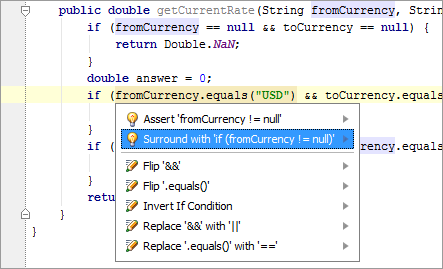
\includegraphics[width=\textwidth]{code_analysis_bugs.png}
%\caption{Рекомендации по проведению исследований в рамках диссертации}%
%\label{fig:how-to-do-research}
%\end{figure}
%
%\Blindtext
%
%\begin{table}
%% Для таблиц с multirow и multicol необходимо вручную указать сдвиг для caption
%\captionsetup{skip=5pt}
%\caption{Example}
%\centering
%\begin{tabular}{|r|c|c|c|c|c|c|}
%\hline
%            \multirow{2}{*}{}
%           & \multicolumn{2}{c|}{LLVM IR} 
%           & \multicolumn{2}{c|}{PS} 
%           & \multicolumn{2}{c|}{AI} \\ \cline{2-7}
%           & SAT    & UNSAT   & SAT    & UNSAT   & SAT    & UNSAT   \\ \hline
%beanstalkd & 356    & 252     & 360    & 161     & 360    & 247     \\ \hline
%clib       & 599    & 258     & 960    & 234     & 960    & 449     \\ \hline
%\end{tabular}
%\label{table:checkResults}
%\end{table}
%
%%%%%%%%%%%%%%%%%%%%%%%%%%%%%%%%%%%%%%%%%%%%%%%%%%%%%%%%%%%%%%%%%%%%%%%%%%%%%%%%%
%\section{bar}
%%%%%%%%%%%%%%%%%%%%%%%%%%%%%%%%%%%%%%%%%%%%%%%%%%%%%%%%%%%%%%%%%%%%%%%%%%%%%%%%%
%
%\blindtext
%It is of great importance that you use correct references in your dissertation.
%Resent studies show that it can increase the chances of successful defense
%by as much as 3,17 percent~\cite{russian, ANTLR, java-book}.
%
%\begin{table}[H]
%	\caption{Название таблицы}
%	\begin{center}
%		\begin{tabular}{|l|l|}
%			\hline
%			top left & top right\\ \hline
%			bot left & bot right\\ \hline
%		\end{tabular}
%		\label{tabular:tab_examp}
%	\end{center}
%\end{table}
%
%
%\Blindtext
